\documentclass{isprs} 

\usepackage{subfigure}
\usepackage{setspace}
\usepackage{geometry}
\usepackage[labelsep=period]{caption}  
\usepackage[british]{babel} 

\usepackage{natbib}
\usepackage{amsfonts,amsmath,bm,bbm}
\usepackage{hyperref} 
\usepackage{graphicx,url}
\usepackage{rotating}

\geometry{a4paper, top=25mm, left=20mm, right=20mm, bottom=25mm, headsep=10mm, footskip=12mm}

\captionsetup{justification=centering,font=normal} 
\captionsetup[figure]{font=small}

\usepackage{color}

\hyphenation{}

\begin{document}

\title{CHARACTERIZATION OF SAR IMAGES WITH WEIGHTED AMPLITUDE TRANSITION GRAPHS}

\author{
	Eduarda T.\ C.\ Chagas\textsuperscript{1}, 
	Alejandro C.\ Frery\textsuperscript{2}\thanks{Corresponding author}, , 
	Osvaldo A.\ Rosso\textsuperscript{3}
	Heitor S.\ Ramos\textsuperscript{1}
}

\address{
	\textsuperscript{1 }Dept.\ of Computer Science, Federal University of Minas Gerais, Belo Horizonte, Minas Gerais -- (eduarda.chagas, ramosh)@dcc.ufmg.br,\\
	\textsuperscript{2 } Laborat\'orio de Computa\c c\~ao Cient\'ifica e An\'alise Num\'erica -- LaCCAN, Universidade Federal de Alagoas, Brasil -- acfrery@laccan.ufal.br\\
	\textsuperscript{3 }Instituto de F\'isica, Universidade Federal de Alagoas, Brasil -- oarosso@if.ufal.br
}

\icwg{}   

\abstract{
	We propose a new technique for SAR image texture characterization based on ordinal pattern transition graphs.
	The proposal consists in
	(i)~transforming a 2D patch of data into a time series using a Hilbert Space Filling Curve,
	(ii)~building an Ordinal Pattern Transition Graph with weighted edges;
	(iii)~obtaining a probability distribution function from this graph;
	(iv)~computing the Entropy and Statistical Complexity of this distribution.
	The weight of the edges is related to the absolute difference of observations.
	This modification takes into account the scattering properties of the target, and leads to a good characterization of several types of textures.
	Experiments with data from Munich urban areas, Guatemala forest regions, and Cape Canaveral ocean samples demonstrate the effectiveness of our technique, which achieves satisfactory levels of separability.
}


\keywords{Synthetic Aperture Radar (SAR), Time-series, Terrain Classification, Permutation Entropy, Ordinal Patterns Transition Graphs, Causality Complexity-Entropy Plane}

\maketitle

\section{INTRODUCTION}\label{Intro}

Surface classification and land use are among the most important applications of Synthetic Aperture Radar (SAR) imaging~\citep{Pottier2004Unsupervised}, for which supervised and unsupervised classification algorithms have been proposed~\citep{Bhattacharya2018Unsupervised,Chen1996multifrequency,ZYL1992Bayesian}.

Classification techniques rely on the extraction and analysis of features from the data, and from additional information and prior knowledge about both the scene, the sensor and the acquisition conditions.
Texture is among the features that carries most information and, as such, it is important to characterize it in a quantitative manner.

The texture in SAR images is characterized twofold, namely by the marginal properties of the data~\citep{adrian96}, and by their spatial structure~\citep{FeaturesCropDiscrimination}.
In this work we focus on the second approach.

The most widely used approach to obtain textural features from SAR imagery is through co-ocurrence matrices and Haralick's descriptors~\citep{Zakeri2017Texture}.
Other approaches include the Fourier power spectrum~\citep{Florindo2012Fractal}, and
Markov random fields~\citep{Deng2005UnsupervisedSO}.

We opt for linearizing image patches into a time series, converting them to weighted graphs, and then extracting information-theoretic features.
With this approach we obtain good discrimination between different types of targets.

The article was divided as follows:
Section~\ref{methodology} presents the proposed methodology.
Section~\ref{linearization} reports how the patch linearization process of the images occurs.
Section~\ref{WATG} describes our technique of ordinal amplitude transition graph weighting by amplitudes.
In Section~\ref{HC} we report the Information Theory descriptors used throughout this work.
Section~\ref{SAR} shows the results obtained in characterizing textures.
We present our conclusions in Section~\ref{Conclusion}.

\section{Methodology}\label{methodology}

Our procedure consists of the following steps:
\begin{enumerate}
	\item\label{item:Linearlize} transforming a 2D patch of data into a time series using a Hilbert Space Filling Curve,
	\item\label{item:WOPTG} building an Ordinal Pattern Transition Graph with weighted edges;
	\item\label{item:Probability} obtaining a probability distribution function from this graph;
	\item\label{item:Descriptors} computing the Entropy and Statistical Complexity of this distribution.
\end{enumerate}
The technique is illustrated in Fig~\ref{fig:WATG}, and detailed in the following.

\begin{figure}[hbt]
	\centering
	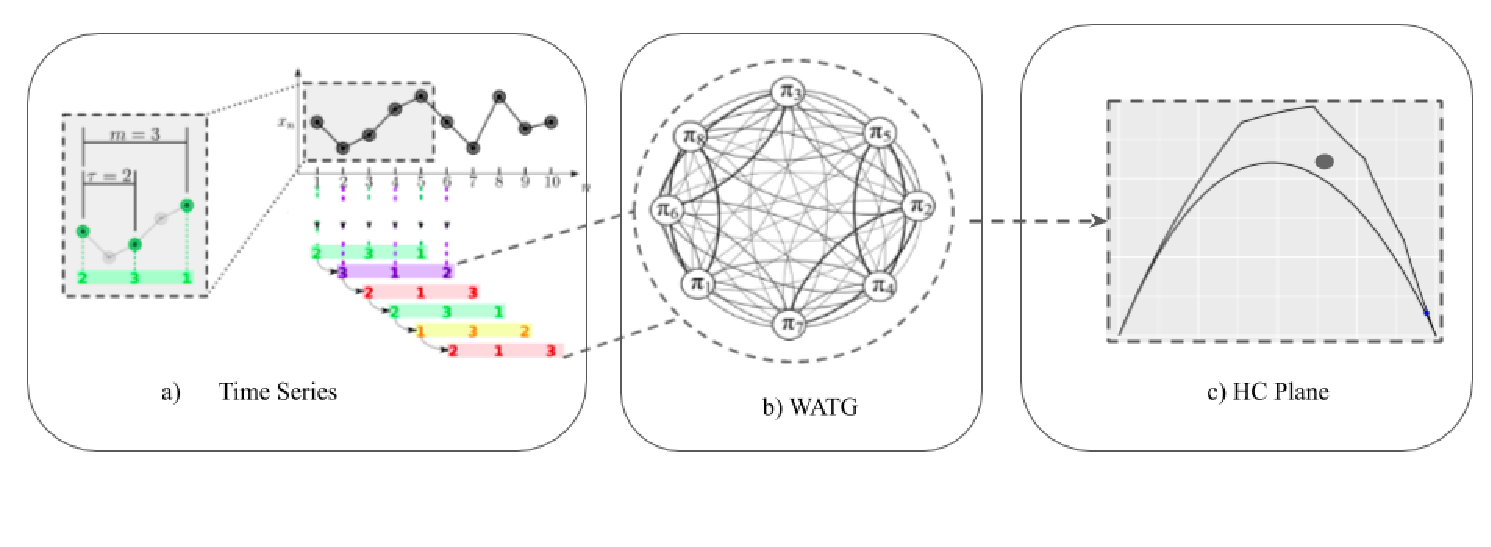
\includegraphics[scale = 0.25]{Figures/WATG.pdf}
	\caption{Outline of the tecnique for the characterization of textures.}
	\label{fig:WATG}
\end{figure}

\subsection{Linearization of image patches}\label{linearization}

The technique is adequate for analyzing time series, therefore the need to transform 2-D patches into 1-D signals.
This could be accomplished by reading the data by lines, columns or any transformation.
In Step~\ref{item:Linearlize} we employ a Hilbert Space Filling Curve~\citep{Lee1994Texture}.

Space filling curves were first employed by Nguyen and Quinqueton (1982), to map a texture into a one-dimensional signal.
When used as scanning methods of an image, such functions preserve relevant properties of pixel spatial correlation~\citep{Lee1994Texture}.

Assuming an image patch is supported by a $N \times N$ dimension grid, where $N$ is a power of $2$, we have the following definition.

\newtheorem{mydef}{Definition}
\begin{mydef}
	An image scan is a bijector function $f \colon \mathbb{N} \times \mathbb{N} \to \mathbb{N}$ in the ordered pair set $ \{(i, j): 1 \leq i , j \leq N \}$, which denotes the points in the domain, for the closed range of integers $\{1, \dots, N^2\}$. Equivalently, the image is encoded by scanning $f$ at pixel intensities in the order $P_{f^{-1}(1)}, P_{f^{-1}(2)}, \dots, P_{f^{-1}(N^2)}$, where $P_{(i, j)}$ represents the pixel strength of column $i$ and row $j$.
	\label{def:CurveFilling}
\end{mydef}

Space filling curves, such as raster-1, raster-2 and Hilbert scanning techniques stipulate a proper function $f$.
As can also be seen from Definition~\ref{def:CurveFilling}, curves impose on us the condition that each pixel is visited only once.


A Hilbert curve is a continuous fractal space fill curve described as a variant of Peano space fill curves.
Such a curve scans an array of pixels with a size of 2m x 2m pixels without ever maintaining the same direction for more than three consecutive points, so that each pixel in a grid is traversed once and only once, as illustrated in Fig~\ref{fig:Hilbert}.
By using the Hilbert curve we can maintain spatial dependence information of the analyzed textures.

\begin{figure}[hbt]
	\centering
	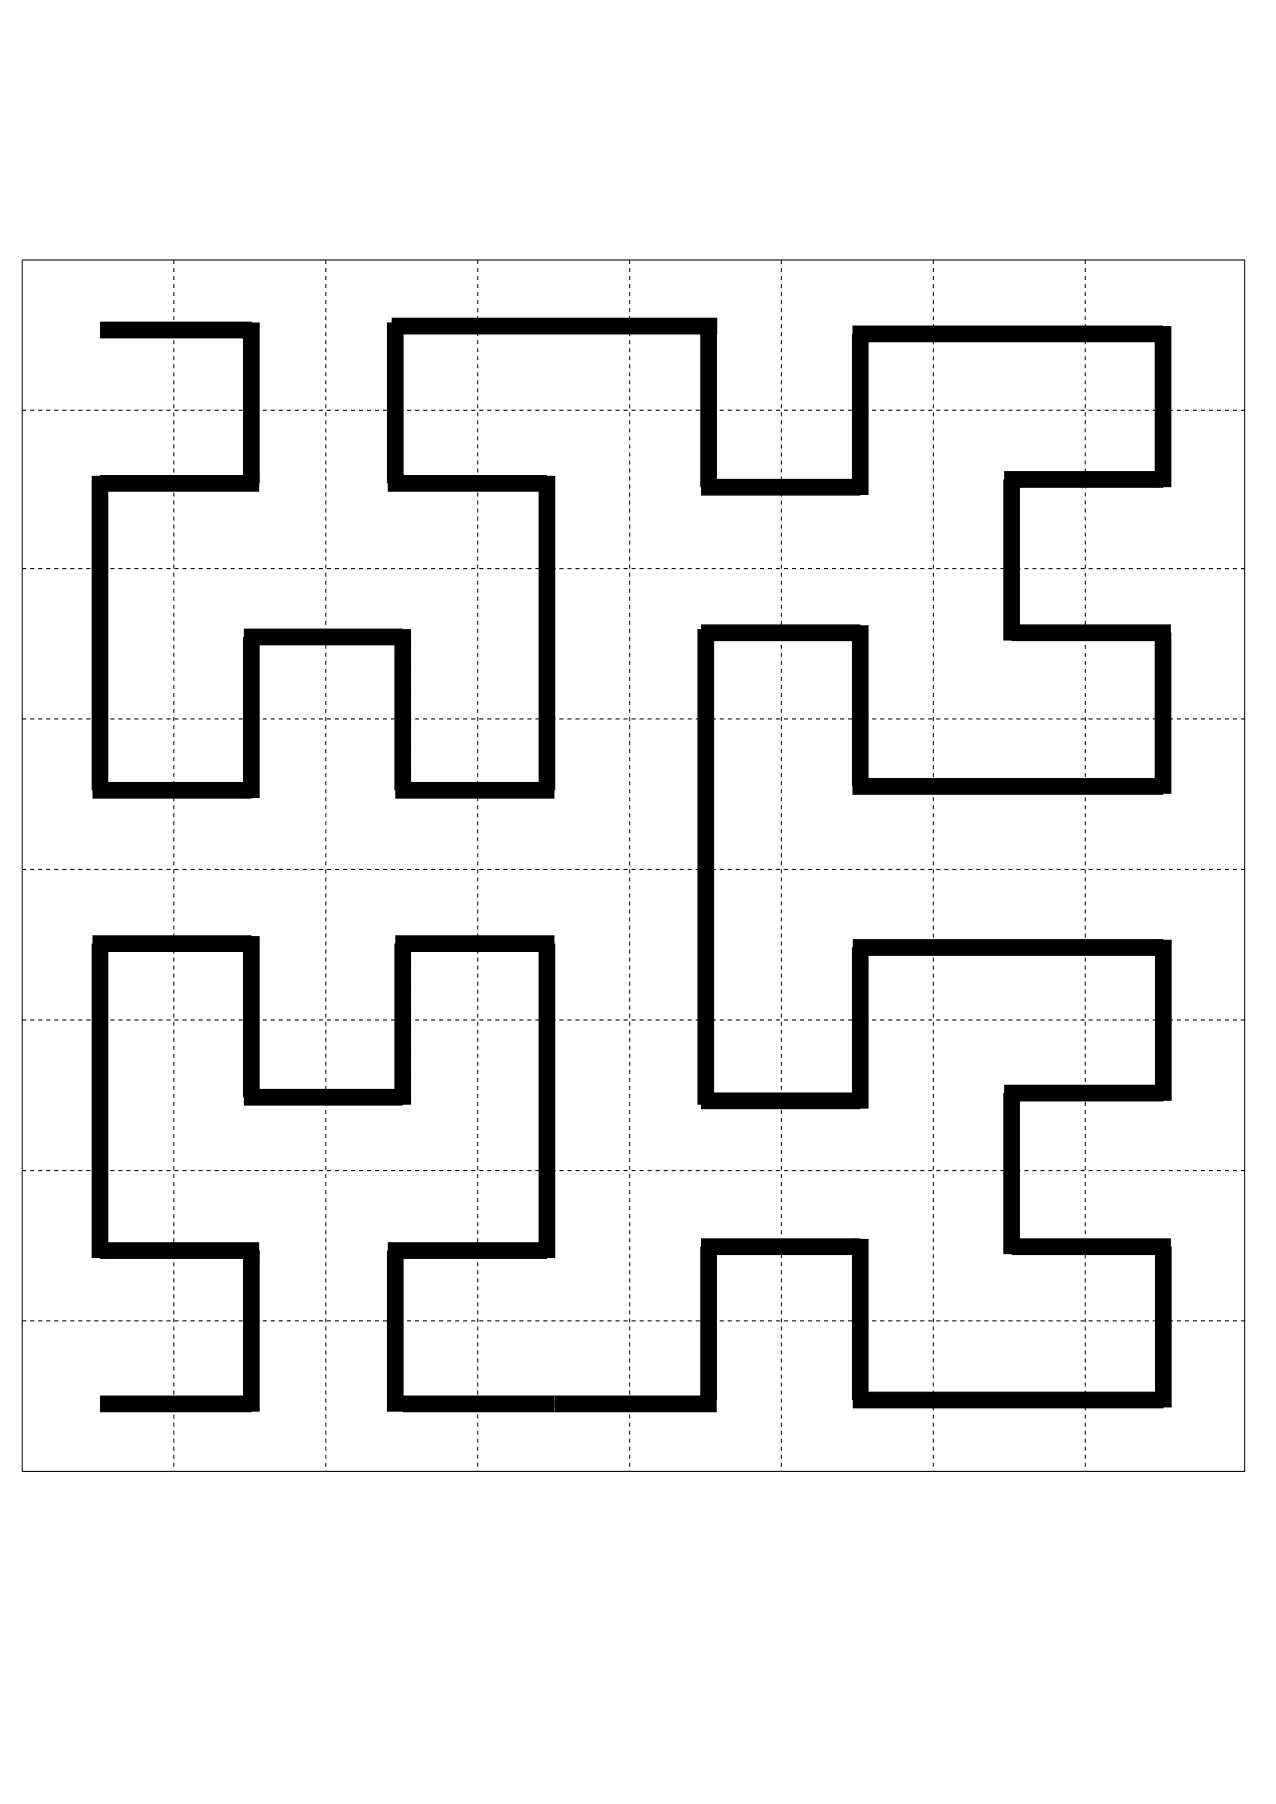
\includegraphics[width=.3\linewidth]{Figures/hilbert.png}
	\caption{The $8 x 8$ window of Hilbert Space Filling Curve scan}
	\label{fig:Hilbert}
\end{figure}

\subsection{Weighted Ordinal Patterns Transition Graph}\label{WATG}

Step~\ref{item:WOPTG} consists of two stages.
In the first, the time series is transformed into a sequence of ordinal patterns.
In the second, we build a weighted graph describing the transitions between these patterns.

The representation by ordinal patterns was introduced by~\cite{Bandt2002Permutation} as a resistant to noise contamination effects, and invariant to linear and nonlinear monotonic transformations.
This representation captures the temporal causality of the data, and reveals important details of the ordinal structure of the time series~\citep{Larrondo2006Random}.

Consider the finite time series of discrete time real values $\mathbb{X} = (x_1, x_2, \dots, x_T)$ with length $T$.
The $\mathbb{X}_t^{m, \tau} $ symbols or words produced at each instant $t = 1, \dots, T- (m-1) \tau$ are given by an embedding dimension $m \in \mathbb{N}$ and a time delay $\tau \in \mathbb{N}$ between patterns as:
\begin{equation}
\mathbb{X}_t^{m,\tau} = (x_{(t-1)+\tau}, x_{(t-1)+\tau+1},\ldots, x_{(t-1)+\tau+(m-1)}).
\end{equation}

The set of ordinal patterns $\pi = \{\pi_t^m: t = 1, \dots, T- (m-1) \tau \}$ are obtained by mapping $\mathbb{X}^{m, \tau}_t \mapsto \pi^m$ by a permutation process of the elements, such that they are sorted in increasing order~\citep{Ravetti2014noise}:
$$
x_{(t-1) + \tau} \leq x_{(t-1) + \tau + 1} \leq \dots \leq x_{(t-1) + \tau + (m-1)}.
$$

The classical approach consists in analyzing the histogram of these patters.
Alternatively, one may form an oriented graph with the transitions from $\pi_t^m$ to $\pi_{t+1}^m$.
We modify this last approach by assigning weights to the edges related to the absolute difference of the observations.
This modification takes into account the scattering properties of the target, and leads to a good characterization of several types of textures.

Denote $\Pi$ the sequence of symbols obtained by a given series $\mathbb{X}_t^{m,\tau}$.
The Bandt-Pompe probability distribution is the relative frequency of symbols in the series against $m!$ possible permutations of patterns $\{\pi_t^m \}_{t = 1}^{m!}$:
\begin{equation}
p(\pi_i^m) = \frac{\#\left \{t : t = 1, \dots, T-(m-1)\tau; \mathbb{X}_t^{m,\tau} \text{ type } \pi_i^m\right \}}{T- (m-1)\tau},  
\end{equation}
that meets the conditions $p(\pi_i^m) \ge 0$ and  $\sum_{i=1}^{m!} p(\pi_i^m) = 1$.

The Ordinal Pattern Transition Graph $\vec{G}_{\pi} = (\vec{V}, \vec{E})$ represents the transitions between two consecutive ordinal patterns over time $t$.
In this new representation, the patterns $\{\pi_t^m \}_{t = 1}^{m!}$ are the vertices of the set $\vec{V} = \{v_{\pi_i}: i = 1, \dots, m! \}$, and the edges $\vec{E} = \{(v_{\pi_i}, v_{\pi_j}): v_{\pi_i}, v_{\pi_j} \in V \}$ indicate the sequential occurrence of two ordinal patterns.

Recent work proposes a weighting in the calculation of relative frequencies for ordinal patterns with different amplitude variances, making them contribute differently to the final value of permutation entropy (PE) and thus incorporating amplitude change information within a given set~\citep{Fadlallah2013Weightedpermutation}.
However, these methods do not consider the amplitude difference present in different time series, weighing them similarly when calculating the final value of their probabilities.
Therefore, data with different amplitudes but with similar variance dynamics are not discriminated, losing important information about the system dynamics.

To counterbalance these facts, we propose a modification of the current ordinal pattern transition graph by incorporating meaningful time series information.

Two approaches are considered in relation to the weight of edges in the literature.
Some authors employ unweighted edge~\citep{McCullough2015lagged, Kulp2016ordinal} representing only the existence of such transitions, while others apply the frequency of transitions~\citep{Sorrentino2015periodic, Zhang2017ConstructingOP}.
The weights $\mathbb{W} = \{w_{v_{\pi_i}, v_{\pi_j}}: v_{\pi_i}, v_{\pi_j} \in V \}$ assigned to each edge describes the chances of transition between two particular patterns $(v_{\pi_i}, v_{\pi_j})$ calculated by their respective relative frequencies, ie:	
\begin{equation}
w_{v_{\pi_i}, v_{\pi_j}} = \frac{|\Pi_{\pi_i,\pi_j}|}{m-1},
\end{equation}
where $|\Pi_{\pi_i,\pi_j}|$ is the number of transitions from pattern $\pi_i$ to pattern $\pi_j$ and $\sum_{v_{\pi_i}, v_{\pi_j}}w_{v_{\pi_i}, v_{\pi_j}} = 1$.

Our proposal, henceforth referred to as Weighted Amplitude Transition Graph (WATG), incorporates the absolute difference between the observations that produced the patters.

First, each $\mathbb{X}$ time series is scaled to $[0, 1]$, since we are interested in a metric able to compare data sets:
\begin{equation}
x_{\text{new}} = \frac{x - x_{\min}}{x_{\max} - x_{\min}},
\end{equation}
where $x_{\min}$ and $x_{\max}$ are, respectively, the minimum and maximum values of the series.

Each $\mathbb{X}^{m, \tau}_t$ vector is associated with a weight $\beta_t$ that measures the largest difference between its elements:
\begin{equation}
\beta_t = \max\{x_i - x_j\},
\end{equation}
where $x_i, x_j \in \mathbb{X}^{m, \tau}_t$.

Traditionally, the transition graph assigns uniform weight to each transition between patterns and normalizes the result obtained by dividing by the total transitions.
In this modification, the $w_{v_{\pi_i}, v_{\pi_j}}$ weights assigned to each edge depict the amplitude difference observed in the transition.
So we have that:	
\begin{equation}
w_{v_{\pi_i}, v_{\pi_j}} =  \sum_{i : \{\mathbb{X}^{m,\tau}_t \mapsto \pi_i\}} \sum_{j : \{\mathbb{X}^{m,\tau}_t \mapsto \pi_j\}} |\beta_i - \beta_j| .
\end{equation}

Thus, the probability distribution taken from the weighted amplitude transition graph is given as follows:	
\begin{align}
&\left\{\begin{array}{l}
\lambda_{v_{\pi_i}, v_{\pi_j}} = 1, \text{ if } (v_{\pi_i}, v_{\pi_j}) \in \vec{E} \\
\lambda_{v_{\pi_i}, v_{\pi_j}} = 0, \text{ otherwise}.
\end{array}\right. \\
%
&p(\pi_i, \pi_j) = \frac{\lambda_{v_{\pi_i}, v_{\pi_j}} . w_{v_{\pi_i}, v_{\pi_j}}}{\sum_{v_{\pi_a}, v_{\pi_b}} w_{v_{\pi_a}, v_{\pi_b}}}.
\end{align}
Note that the conditions $p(\pi_i, \pi_j) \ge 0$ e $\sum_{\pi_i, \pi_j} p(\pi_i, \pi_j) = 1$ are satisfied.

Thus, series with uniform amplitudes have edges with probability of occurrence well distributed along the graph, while those with small amplitude and large peaks have edges with probability of occurrence much higher than the others.

\subsection{Information-Theoretic Descriptors}\label{HC}

Entropy measures the disorder or unpredictability of a system characterized by a probability measure $\mathbb{P}$.

Let $\mathbb{P} = \{p_{(\pi_1, \pi_1)}, p_{(\pi_1, \pi_2)}, \dots, p_{(\pi_{m!}, \Pi_{m!})} \}$ be the probability distribution taken from the time series weighted amplitude transition graph $\mathbb{X}$.
The Shannon entropy is given by:	
\begin{equation}
H(\mathbb{P}) = -\sum_{i=1}^{m!m!} p_i \log p_i .
\label{eq:Entropia}
\end{equation}

The ability of the entropy to capture system properties is limited, so it is necessary to use it in conjunction with other descriptors to perform a more complete analysis.
Other interesting measures are distances between the $\mathbb{P}$ probability function and a probability measure that describes a non-informative process, typically the uniform distribution.

The Jensen-Shannon distance to the uniform distribution $\mathbb{U} = (\frac{1}{m!m!}, \dots, \frac{1}{m!m!})$ is a measure of how similar the underlying dynamics are to a process without information; it is calculated as:
\begin{equation}
D(\mathbb{P}, \mathbb{U}) = \sum_{i=1}^{m!m!} \Big(p_i \log\frac{p_i}{u_i} +
u_i \log\frac{u_i}{p_i}
\Big).
\end{equation}
This quantity is also called ``disequilibrium.''

Conversely to entropy, statistical complexity seeks to find interaction and dependence structures among the elements of a given series, being an extremely important factor in the study of dynamic systems.

This quantity is defined using the expression given by \citet{Lopez1995statistical}, 
that combines an Entropy and a Distance, yielding the Statistical Complexity~\citep{Feldman2008information,Feldman1998Statistical}:
\begin{equation}
C(\mathbb{P}, \mathbb{U}) = H(\mathbb{P}) D(\mathbb{P}, \mathbb{U}).
\end{equation}

Each time series can then be described by a point $(H(\mathbb{P}), C(\mathbb{P}, \mathbb{U}))$.
The set of all pairs $(H(\mathbb{P}), C(\mathbb{P}, \mathbb{U}))$ for any time series described by patterns of length $m$ lies in a compact subset of $\mathbbm R^2$: the Entropy-Complexity plane. 

Through such a tool it is possible to discover the nature of the series, determining if it corresponds to a chaotic, stochastic or deterministic sequence.

\section{TEXTURAL CLASSIFICATION OF SAR REGIONS}\label{SAR}

Widely used in recognizing geographical features and patterns, synthetic aperture radar (SAR) images are rich in texture information. 
For this analysis we used three images SAR with different regions:
\begin{itemize}
	\item Sierra del Lacandon National Park, Guatemala (acquired on April 10, 2015), available at \url{https://uavsar.jpl.nasa.gov/cgi-bin/product.pl?jobName=Lacand_30202_15043_006_150410_L090_CX_01#dados};
	\item Cape Canaveral Ocean Regions (acquired September 22, 2016);
	\item Urban area of the city of Munich, Germany (acquired June 5, 2015).
\end{itemize}
%%% ACF O sensor é o mesmo? Aqui dar detalhes, dizer que usamos HH em intensidade

We used $160$ samples of size $128\times128$: $40$ samples from each category of regions, namely,
Guatemalan forest regions; 
Type~1 oceanic regions of Cape Canaveral; 
Type~2 oceanic regions of Cape Canaveral; and 
urban regions of the city of Munich. 
Figure~\ref{fig:RegioesSAR} shows examples of each of them.

\begin{figure}[hbt]
	\centering
	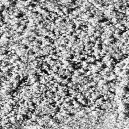
\includegraphics[width=.23\linewidth]{Figures/guatemalaflorest}
	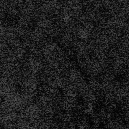
\includegraphics[width=.23\linewidth]{Figures/Cape1}
	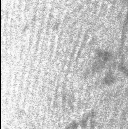
\includegraphics[width=.23\linewidth]{Figures/Cape2}
	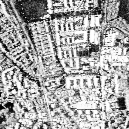
\includegraphics[width=.23\linewidth]{Figures/munichUrban}	
	\caption{Types of regions analyzed: Forest, Sea Type~1, Sea Type~2, and Urban.}\label{fig:RegioesSAR}
\end{figure} 

Since the symbolization process is invariant to monotonous transformations and resistant to contamination effects, contrast changes are not capable of causing changes in the final results obtained by the descriptors.
%%% ACF Não entendi o que segue. Se você juntou Type~1 e Type~2, não comece dizendo que são duas classes.
Thus, the different types of oceanic regions considered in this study were studied as a single more general class.

%Data resulting from remote sensing have a peculiar feature that justifies the application in this article:
%The intensities of an image and hence the amplitude difference in the data classes depend on the properties of the target we are analyzing due to the backscatter properties.
%Thus, urban targets are those that usually give the highest returns, followed by forests, and finally, water bodies, as can be seen in the figure~\ref{fig:AmplitudeSAR}.

%Therefore, in this paper we aim to represent, through the weighted amplitude transition graph, to model this amplitude difference in the probability distribution of our data.
%The analysis methodology proposed and applied to the texture data set SAR can be seen in the figure~\ref{fig:WATG}.

Fig.~\ref{fig:AmplitudeSAR} shows examples of forest, sea and urban samples as time series.

\begin{figure}[hbt]
	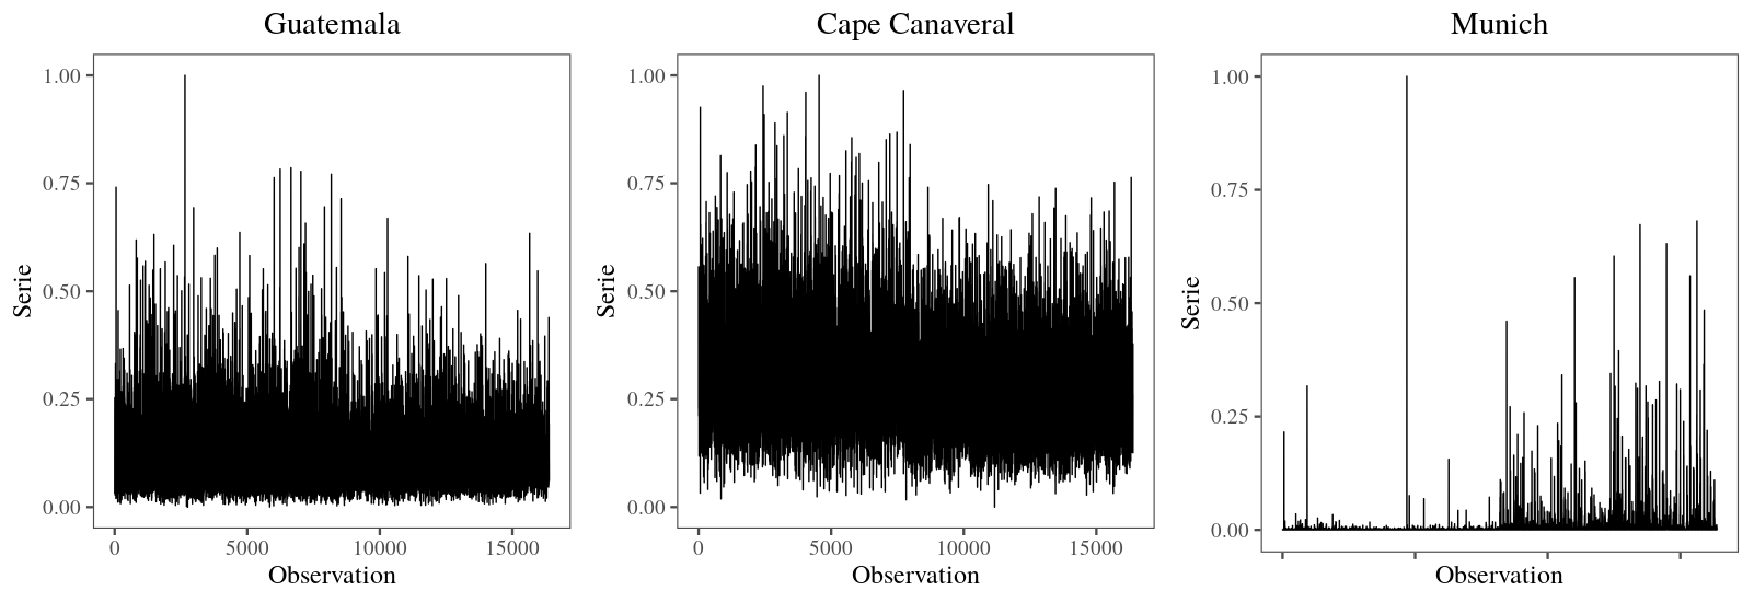
\includegraphics[width=\columnwidth]{Figures/SAR_signal.pdf}
	\caption{Analysis of the amplitude of the different types of regions: (a) Oceanic Region; (b) Forest Regions and (c) Urban Regions}
	\label{fig:AmplitudeSAR}
\end{figure}

%After linearizing the textures using the Hilbert curve, we used the sliding window technique to obtain our symbols, thus:
%\begin{equation}
%\mathbb{X}_t^{m,\tau} = (x_{t}, x_{t+\tau},\ldots, x_{t+(m-2)\tau} ,x_{t+(m-1)\tau}).
%\end{equation}

Fig.~\ref{fig:Regions} shows the results for several dimension values $m$ and delays $\tau$.
Since such values inform us of intrinsic characteristics of the dynamics of the series in their specific domains, inadequate values may hide this kind of knowledge about the data, and this analysis step is extremely crucial.
We obtained the best characterization with $\tau = 1$.

\begin{sidewaysfigure*}
	\centering
	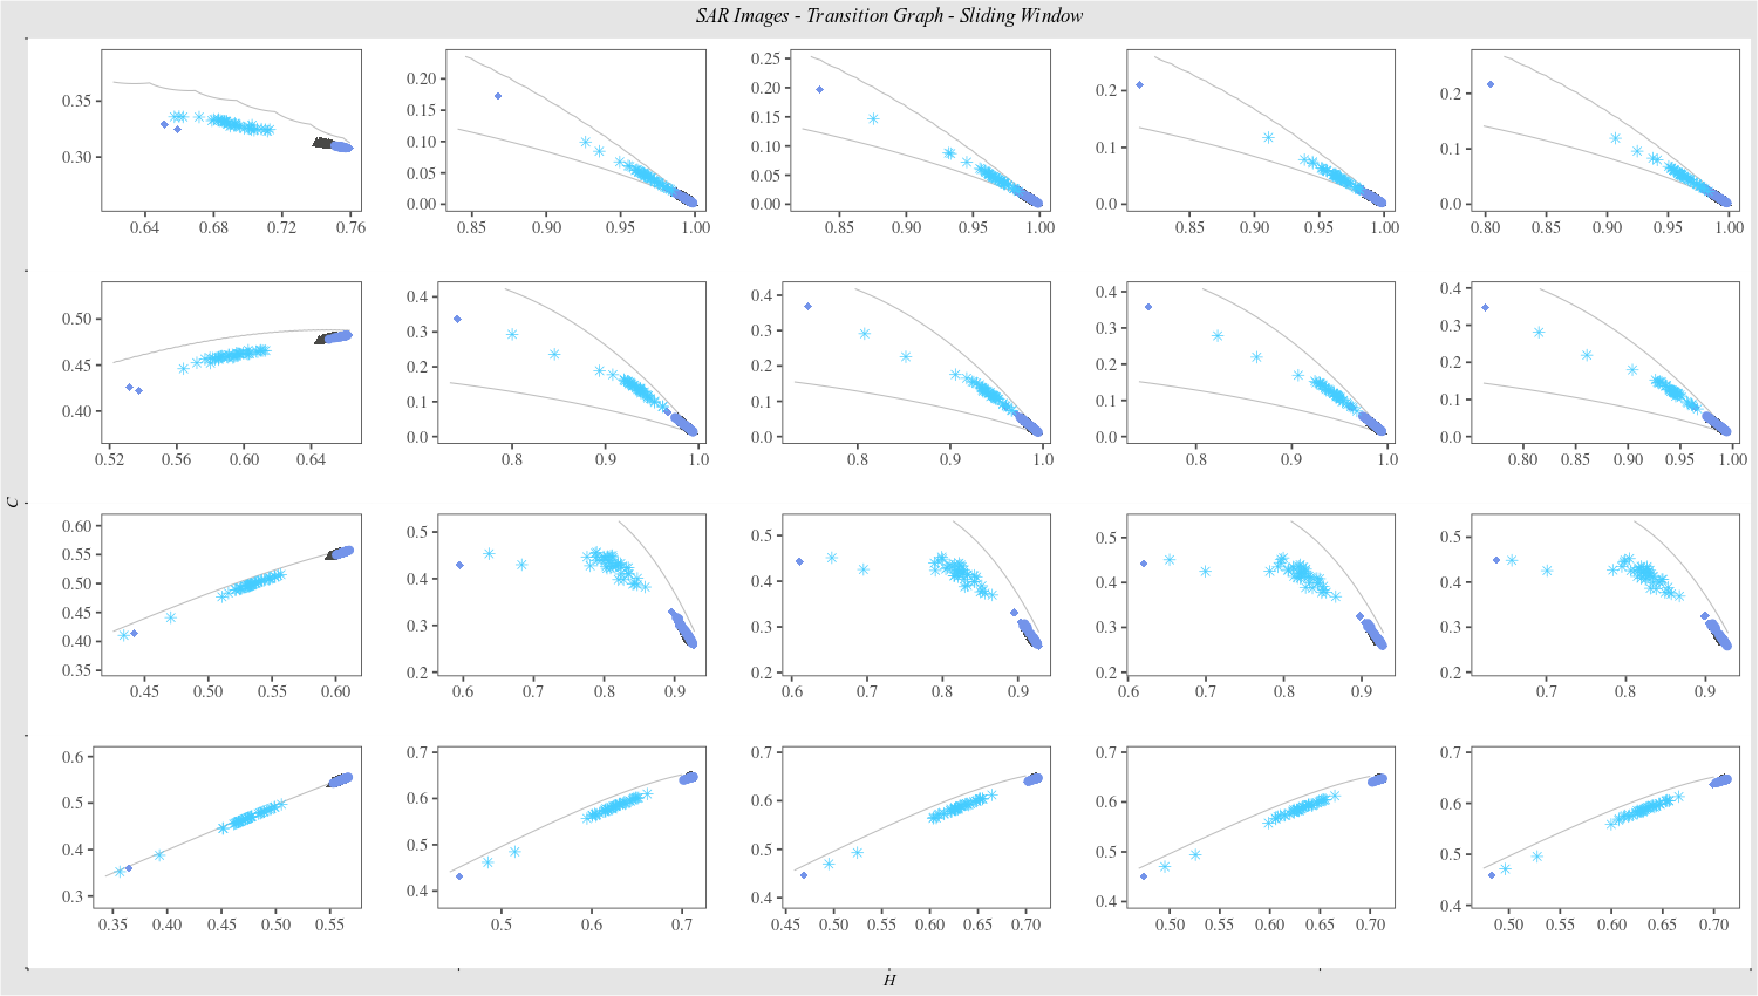
\includegraphics[width=1.05\textwidth]{Figures/transitionGraphHilbert.pdf}
	\caption{Characterization resulting from the application of the \texttt{Hilbert curve} in WATG on textures of different regions: Guatemala (Green), Cape Canaveral (Blue) and Munich (violet). Charts evolve horizontally according to the $m$ dimension chosen and vertically with the delay $\tau$}
	\label{fig:Regions}
\end{sidewaysfigure*}

%%% ACF Caso haja espaço, mostrar o melhor resultado e analisá-lo


\section{CONCLUSION}\label{Conclusion}

We proposed a new weighting technique in the formation of Ordinal Pattern Transition Graphs.
The edge weights are proportional to the amplitude variations during the transitions.
%Thus, the closer the entropy $\mathbb{H}$ is to $0$ the more uniform the probability distribution $\mathbb{P}$ will be, informing us that the series does not have large amplitude variances.
%However, if a series has a low amplitude but has large variations (peaks) over time, WATG will be able to infer such behavior by placing a greater weight on these transitions, making the entropy $\mathbb{H}$ approach $1$.

To test the proposed technique we performed the characterization of different regions in textures of SAR images.

As a result, in addition to perfectly separating urban areas from the others analyzed by entropy values, we are still able to differentiate oceanic and forest areas through their different values of statistical complexity, which informs us of the degree of temporal dependence between their elements.

\bibliographystyle{isprs}
\bibliography{../../Common/references.bib}

\section*{ACKNOWLEDGEMENTS}\label{ACKNOWLEDGEMENTS}

This work was partially funded by the Coordination for the Improvement of Higher Education Personnel (CAPES).


\end{document}